\documentclass[11pt,a4paper,twocolumn]{article}
% -*-mode: tex;coding: utf-8;-*-

% direkt input of umlauts
\usepackage[utf8]{inputenc}
% use standard PS-Font
\usepackage{times}
% narrower border
\usepackage[colorlinks=false, pdfborder={0 0 0}]{hyperref}
% enable [b] placement option for twocolumn figures (figure*)
\usepackage{stfloats}

\usepackage{subeqn}
\usepackage{listings}

% make description item font customizable
\usepackage{enumitem}

% customize figure and table captions
\usepackage[font=small,margin=1ex,labelfont=bf]{caption}

% subfigures
\usepackage{subfigure}
%\subfigtopskip=0pt
%\subfigcapskip=0pt
%\subfigbottomskip=0pt

\usepackage{algorithm}
\usepackage[noend]{algpseudocode}



% page layout
\usepackage{calc}
\usepackage[left=2.0cm,right=2.0cm,top=3.0cm,bottom=3.0cm]{geometry}

% comment out for English:
\usepackage[ngerman]{babel}

% vspace rather than paragraph indention
\usepackage{parskip}
% no extra space after periods
\frenchspacing

% avoid words crossing right border
\tolerance=9000

\usepackage{graphicx}

\usepackage{float}
% Header and footer
%=======================================================================
\usepackage{fancyhdr}
\pagestyle{fancy}
% ersetzen:
\lhead{Energieeffizienzanalyse}
%% \chead{}
\rhead{Wahlpflicht-Projekt WS 2018/2019}
\renewcommand{\footrulewidth}{0pt}

% pagestyle on first page
\fancypagestyle{firstpage}{
  \fancyhead{}
  \cfoot{\footnotesize{\em Wahlpflicht-Projekt WS 2018/2019, Hochschule Niederrhein, Fachbereich Elektrotechnik \& Informatik}}
  \renewcommand{\headrulewidth}{0pt}
}

% Title
%=======================================================================
% Ersetzen durch Titel des Vortrags:
\title{\vspace*{-10mm}Projekt Energieeffizienzanalyse}
\author{
% Autor und Email-Adresse ersetzen:
Team Energieeffizienzanalyse\\
Hochschule Niederrhein\\
Fachbereich Elektrotechnik und Informatik\\
Reinarzstr. 49, 47805 Krefeld
}
\date{}

%
%=======================================================================
\begin{document}

% a), b), c) fur subitems
%\renewcommand{\labelenumi}{\alph{enumi})}
\renewcommand{\labelenumi}{\arabic{enumi})}

%\thispagestyle{empty}

\twocolumn[
	\begin{@twocolumnfalse}
		\maketitle
		\begin{abstract}
			%!TEX root = ../paper.tex

% \noindent Die Hauptaufgabe des Projektes war die Interpolation von Lastgängen. Der Projektbericht gibt einen Überblick darüber, wie die Realisierung dieser Aufgabe durch das Projektteam gestaltet wurde. Dabei geht er zunächst darauf ein, warum eine Interpolation notwendig ist, und es werden Überlegungen getroffen, wie sich diese bedarfsgerecht realisieren lässt. Anschließend werden mehrere Algorithmen vorgestellt, angefangen von einfachen Verhältnis-Matrizen über lineare und polynomiale Verfahren bis hin zu Datenbankansätzen. Zusätzlich zu den Algorithmen werden Überlegungen zu Heuristiken vorgestellt, die entweder ergänzend zu den Algorithmen oder gar eigenständig Werte generieren können. Danach werden dann alle möglichen Algorithmen und Heuristiken miteinander auf verschiedenen Testdaten verglichen und auch bewertet. Zu guter Letzt folgt ein Ausblick: Die Tests und Bewertungen der Algorithmen, aber auch die Verfahren selbst, können durch die Verfügbarkeit weiterer Lastgänge deutlich verbessert werden. Auch wird auf komplexere Algorithmen und neuronale Netze als Alternative hingewiesen.

\noindent Zur Bewertung der Rentabilität einer Solaranlage ist die Kenntnis der Stromverbräuche für detaillierte zeitliche Intervalle notwendig. In Abhängigkeit der Deckung von Erzeugung und Verbrauch des Stroms ergeben sich unterschiedliche Notwendigkeiten zum Einkauf externen Stroms. Bei der Aufzeichnung des Energieverbrauchs kann es aufgrund zahlreicher Probleme zu Ausfällen kommen.
Das Projekt befasst sich wesentlich mit der Vervollständigung dieser fehlenden Werte. Dabei wurden mathematische Ansätze, unter anderem eine Interpolation nach dem Newton-Verfahren, und wissensbasierte Verfahren, die naheliegende vorhandene Werte oder die Messwerte anderer Datensätze verwenden, eingesetzt. Die Evaluation der Algorithmen ergab gerade bei großen Datenlücken gute Ergebnisse der wissensbasierten Ansätze.
		\end{abstract}
		\vspace*{5ex}
	\end{@twocolumnfalse}
]
\thispagestyle{firstpage}

%-----------------------------------------------------------------------
%!TEX root = ../paper.tex

\section{Aufgabe \& Motivation}

Im Laufe dieses Berichts werden mehrere Algorithmen vorgestellt, die sich mit der Interpolation, also dem Finden einer Funktion zu gegebenen, diskreten Daten, von Werten beschäftigt. Der Ursprung basiert dabei auf einer Masterarbeit, die ausrechnet, ob und wann eine Solaranlage sich rentiert. Dabei werden mithilfe von Algorithmen gegebene Werte (also zum Beispiel Anzahl an Solaranlagen, gedeckter Flächeninhalt und Anschaffungskosten) genommen und diese mit den Lastgängen verglichen. Ein Lastgang ist der Energie- / Stromverbrauch über einen bestimmten Zeitraum. Benutzer sollen in der Lage sein anhand ihrer Lastgänge und ihrer Eingabeparameter möglichst genau zu berechnen, wann und ob sich die Anschaffung einer Solaranlage rentiert. Früher war die Rechnung vergleichsweise einfach - da der Erlös von verkauftem Strom höher war als die Verbrauchskosten von Strom hatte man sämtlichen Strom einfach verkaufen können und konnte so ganz einfach den erzeugten Strom mit dem Verkaufspreis multiplizieren. Mittlerweile werden Solaranlagen allerdings nicht mehr so subventioniert wie es früher war - der Verkaufspreis für Strom ist nun deutlich geringer als der Kaufpreis. Daher ist es sinnvoller, erzeugten Strom selbst zu benutzen, statt ihn zu verkaufen, und den erzeugten Strom dementsprechend nur zu verkaufen, wenn man zu der Zeit der Erzeugung keinen Eigenbedarf hat. Um möglichst vielversprechende Aussagen über die Rentabilität treffen zu können, ist es heute allerdings erforderlich, dass eine solche Gegenüberstellung, also dem Verbrauch anhand von Lastgängen und die Erzeugung von Strom, durchgeführt und diese mit den jeweiligen Faktoren multipliziert wird. Je mehr Lastgänge vorhanden sind, desto genauer ist am Ende die Rentabilitätsrechnung, allerdings kommt es selten vor, dass Verbraucher über längere und lückenlose Zeiträume von Lastgängen verfügen. Es ist eher so, dass wenn ein Verbraucher Lastgänge zur Verfügung hat, dann sind diese meistens begrenzt, z. B. nur für ein halbes Jahr. Auch kann es vorkommen, dass dort mehrere Lücken sind, da das Gerät für ein paar Tage ausgefallen ist oder einen technischen Defekt hatte. Die Hauptaufgabe ist also auf der einen Seite die Interpolation von Werten, um genau diese Lücken zu füllen. Auf der anderen Seite, weil sich Solaranlagen wahrscheinlich nicht in solch kurzer Zeit rentieren, ist es die Erstellung von Prognosen, da der Stromverbrauch zeitlich variable ist: Im Winter wird zum Beispiel deutlich mehr verbraucht als im Sommer. Der letzte Fall ist, dass Verbraucher gar keine Lastgänge zur Verfügung haben. Diesen soll es ermöglicht werden deren Lastgänge anhand eines Profilgenerators zu schätzen.

Für das Projekt liegen uns zwei Lastgänge in Form einer Excel Tabelle vor. Eins vom Jahr 2016, das zweite für das Jahr 2017. Jeweils gegeben ist ein Datum, eine Uhrzeit und der gemessene Wert in kWh und das im 15-Minuten-Takt.
%-----------------------------------------------------------------------

%!TEX root = ../paper.tex

\section{Algorithmen}

Um möglichst gute Interpolationswerte und Prognosen zu erzielen, werden im Folgenden mehrere Algorithmen erstellt und getestet. Am Ende des Berichts wird anhand von Bewertungsverfahren betrachtet, welcher Algorithmus die besten Werte erzeugt. Als beste Werte werden solche betrachtet, die die geringste Abweichung oder auch kleinste euklidische Distanz haben. % HIER noch/schon erwähnen, dass die Bewertung ggf. nicht so vielversprechend ist, weil es der gleiche Lastgang / Haushalt ist?

	%!TEX root = ../paper.tex

\subsection{Korrelationsmatrizen}

Es gibt Verbraucher, die verfügen über keine Lastgänge, wissen allerdings, wie hoch ihr Gesamtverbrauch im Jahr war. Wenn man dieses Wissen jetzt aufteilt auf die einzelnen Monate und ggf. sogar Tage, dann kann daraus ein Lastgang erstellt werden. Die erste Idee ist also das Ermitteln der Abhängigkeiten der Monate von den anderen Monaten. Allgemein ist bekannt, dass im Sommer zum Beispiel ca. zehn bis fünfzehn Prozent weniger verbraucht wird als im Winter. Für einen Lastgang werden allerdings deutlich detailliertere Informationen benötigt - wie fällt zum Beispiel der Unterschied vom Januar zum Februar aus? 

Daher wäre eine Matrix, die die Abhängigkeiten zu den anderen Monaten darstellt, nützlich. Zunächst erstellen wir eine durchschnittliche Stundenvektorliste. Dafür durchlaufen wir die Lastgänge von einem Jahr, entfernen mithilfe des Boxplots Algorithmus starke Ausreißer von jedem Tag, summieren dann alle Verbrauchswerte derselben Stunde (also 00:00, 00:15, 00:30, 00:45) auf und teilen die Summen durch die Anzahl an Werten von der Stunde (vier, wenn keine Werte durch den Boxplot raus gelöscht wurden), sodass wir am Ende eine Vektorliste haben, die pro Tag nur noch 24 hat, statt wie zuvor 96 Werte. Ausreißer bei den 15-Minuten-Werten werden entfernt, da diese den Durchschnitt stark ändern könnten und es sogar kontraproduktiv ist, wenn Werte erfasst werden, bei dem ein Verbraucher zum Beispiel für 3 Minuten alle Elektrogeräte (inkl. Herdplatten, Backoffen, ...) angeschaltet hat, um einen Stresstest auszuführen. Auf der Stundenvektorliste basierend wird jetzt eine Tagesvektorliste erstellt, indem alle Werte von einem Tag addiert und wieder durch Anzahl geteilt werden. Dasselbe wird ebenfalls für die Monatsvektorliste durchgeführt. Dieser Vorgang wird für beide Lastgänge gemacht, die vorhanden sind. 

Der nächste Schritt ist das Erstellen der Korrelationsmatrizen. Auch hier wird der Vorgang identisch für alle Matrizen (und jeweils alle Lastgänge) werden und daher wird nur die Erstellung der Monatsmatrix erläutert. Prinzipiell wird lediglich jeder Monat mit jedem Monat dividiert, sodass man eine 12x12 Matrix hat, die jeweils das Verhältnis von jedem Monat zu allen anderen Monaten beinhaltet. %was folgender Code-Ausschnitt demonstriert:

%\begin{algorithm}
%	\caption{Korrelationsmatrix}\label{alg:euclid}
%	\begin{algorithmic}[1]
%		\Procedure{createCorMatrix}{$MonVekList$}
%		\State $MonatsKorMatrix\gets new Array[12][12]$
%	    \For{\texttt{i = 0 BIS 11}}
%	    	\For{\texttt{j = 0 BIS 11}}
%				\State \texttt{MonatsKorMatrix[i][j] = MonVekList[i] / MonVekList[j]}
%			\EndFor
%		\EndFor
%		\State \textbf{return} $MonatsKorMatrix$
%		\EndProcedure
%	\end{algorithmic}
%\end{algorithm}

Anschließend werden alle Korrelationsmatrizen desselben Typs, also zum Beispiel alle Monatskorrelationsmatrizen, aufaddiert und durch die Anzahl geteilt, um so eine durchschnittliche Korrelationsmatrix zu erstellen. Einzelne Ausreißer wurden zwar durch den Boxplot Algorithmus eliminiert, so kann man aber auch ganze Lastgänge etwas angleichen, denn vermutlich kein Haushalt wird identisch zu den Lastgängen sein, mit denen hier im Projekt gearbeitet werden. Je mehr Lastgänge in diesem Algorithmus eingeflossen werden, desto genauer werden die einzelnen Relationen zwischen den Monaten.

Jetzt ist es möglich einen Gesamtverbrauch von einem Jahr anzugeben und dadurch zu berechnen, wie viel die einzelnen Stunden, Tage, Monate, ... von dem Gesamtverbrauch ausmachen. Das Ergebnis ist allerdings nur eine Annäherung und das, nachdem sehr viele, unterschiedliche Lastgänge verfügbar sind und die in diesen Algorithmus mit einbezogen werden.
	\label{sec:easy_algorithms}
%-----------------------------------------------------------------------


\subsection{Lineare Interpolation}

Bei der Verwendung einer linearen Interpolation werden meistens Fälle betrachtet, in denen sich Lücken zwischen bereits vorhandenen Daten befinden. Dabei wird unterstellt, dass der Verbrauchsverlauf nahezu linear ist. Für jeden Verbrauchszeitpunkt $x$, dessen Verbrauchswert $y$ unbekannt ist, eine Gerade zwischen zwei benachbarte Punkte $x_1$ und $x_2$ gelegt, wobei gilt $x1\leq\ $x $\leq \ x_2$. Für jeden unbekannten Datenpunkt $P(x/y)$, der auf dieser Gerade liegt, ergibt sich die Formel:
$$y = y_1 + \frac{y_2 - y_1}{x_2 - x_1} \cdot (x - x_1)$$
Die lineare Interpolation eignet sich dazu, zu ermitteln, in welchem Wertebereich sich die nicht erfassten Verbrauchswerte befinden können. Die Ergebnisse wurden in diesem Projekt als Vergleichswerte für die verbesserten Interpolations-Algorithmen verwendet, um deren Stabilität und Zuverlässigkeit zu bewerten. Für eine Erfassung der tatsächlichen Verbrauchswerte eignet sich die lineare Interpolation weniger, da zwar ein steter, aber kein glatter Verlauf der Funktion erzeugt wird. Darüber hinaus birgt sie die Problematik, dass sie nur die direkten benachbarten Verbrauchswerte betrachtet und Schwankungen im Verbrauchsverlauf ignoriert.
%-----------------------------------------------------------------------

\subsection{Polynomielle Interpolationsverfahren}
Die fehlenden Verbrauchswerte sollen im Folgenden auf Basis eines mathematischen Verfahrens ermittelt werden, das nicht nur die direkten benachbarten Punkte, sondern den gesamten Verlauf inklusive Schwankungen und Peaks berücksichtigt. Das Ziel ist es, einen möglichst realistischen Energieverbrauch zu rekonstruieren.\\
Hierfür werden polynomielle Interpolationsverfahren verwendet. Es wird ein Polynom gesucht, das exakt durch die bekannten Punkte aus den Messdaten verläuft. Durch die gegebenen Messdaten wird eine Kurve gelegt, um zu $n+1$ verschiedenen Datenpunkten ein Interpolationspolynom maximal $n-ten$ Grades zu finden.

\subsubsection{Interpolation nach Newton}
Für n Stützstellen wird eine Annäherung an die Polynomfunktion vom möglichst kleinen Grad an (bis maximal Grad $n$) durchgeführt. Gesucht ist eine Polynomfunktion für $n+1$ Stützstellen, mit der die fehlenden Verbrauchsdaten beim Zeitpunkt $n+1$ berechnet werden können. Das Interpolationspolynom ist folgendermaßen aufgebaut:
$$p_n(x)=a_0+a_1(x_n-x_0)+...+a_n(x_n-x_0)...(x_n-x_{n-1})$$
Für jeden weiteren fehlenden Messwert zum Zeitpunkt $n+1$ wird die Formel um $a_{n+1}(x_{n+1}-x_{0})...(x_{n+1}-x_{n})$ erweitert. Das hat den Vorteil, dass das Polynom bei nachfolgenden Punkten nicht komplett neu berechnet werden muss und somit Laufzeit eingespart wird, wohingegen vergleichbare Verfahren wie die Interpolation nach Lagrange hingegen das Polynom mit jedem fehlenden Datenpunkt neu aufbauen.\\
Allerdings hat die Interpolation nach Newton deutliche Schwächen: Das Polynom wird mit zunehmendem Grad instabiler und schwingt stark zwischen den Datenpunkten. Dadurch werden unrealistisch hohe oder niedrige Werte erzeugt, die in einem realen Energieverbrauchsverlauf niemals auftreten können. Deshalb sollte auf ein Polynom hohen Grades verzichtet werden.\\
Das nächste Interpolationsverfahren, das im Rahmen des Projektes implementiert wurde, betrachtet deshalb statt des gesamten Verlaufes nur die $n$ nächsten Nachbarn.

\subsubsection{Splines}

%-----------------------------------------------------------------------
	%!TEX root = ../paper.tex

\subsubsection{Durchschnittsbildung}
Eine Erweiterung zur Interpolation aus Daten des Vortages stellt die Durchschnittsbildung dar. Hierbei fließen zusätzlich zum Wert des Vortages zur selben Uhrzeit weitere Werte in definierten Abständen ein. Der Algorithmus unterstützt verschiedenste Kombinationen, eine Möglichkeit ist der Einfluss von Werten im Wochenabstand und Tagesabstand jeweils zur gleichen Uhrzeit und zusätzlich eine definierte Anzahl an direkt umliegenden Werten. Die Anzahl der Werte pro Intervall ist dabei frei wählbar und gilt jeweils gleich in beide Richtungen.

Bereits vorhandene Werte werden nicht interpoliert, sondern übernommen. Bei der Bildung des Durchschnittswerts, der das Interpolationsergebnis darstellt, sind verschiedene Ansätze denkbar. Der einfachste Ansatz ist die einfache Mittelwertbildung, bei der die Summe der Werte durch die Anzahl der Werte geteilt wird. In der Praxis sollten bestimmten Werte jedoch einen höheren Einfluss auf das Ergebnis erhalten als andere, weshalb die Berechnung angepasst wird.
Zum Einen ist eine Gewichtung in Abhängigkeit der Entfernung zum Interpolationszeitpunkt möglich, so dass die äußersten Werte das Ergebnis deutlich weniger beeinflussen als nah am Zeitpunkt liegende Werte.
Auch der Einfluss der Werte verschiedener Intervalle kann unterschiedlich stark sein. Deshalb ist es möglich, jeder Konfiguration für ein Intervall ein Gewicht zuzuweisen, mit dem die Werte multipliziert werden. Die Bestimmung der Summe an Werten wurde dementsprechend angepasst, so dass die Gewichte das Ergebnis nicht verschieben.

Die größte Herausforderung dieses Ansatzes ist die Konfiguration der Interpolationsintervalle. Eine variable Anzahl an Parametergruppen (eine Gruppe pro Intervall) mit zahlreichen einzelnen Parametern muss konfiguriert werden. Hierfür können entweder Fachwissen eingesetzt oder Konfigurationen ausprobiert werden.
Bei sehr großen Lücken sind die Ergebnisse je nach Konfiguration nicht mehr allzu gut, da nur wenige vorhandene Werte in die Berechnung einfließen können.

\subsubsection{Datenbankansatz}
Im Gegensatz zu den anderen Algorithmen, die lediglich gegebene Werte des zu interpolierenden Datensatzes in die Berechnung einfließen lassen, interpoliert der Datenbankansatz Werte auf Basis mehrerer anderer Datensätze, deren Mittelwert fehlende Werte bildet.

Während einer Vorverarbeitungsphase, nach dessen Abschluss beliebig viele Werte interpoliert werden können, wird die Datenbank aus zahlreichen gesammelten Lastprofilen gebildet. Eingenschaften, entweder einfache Attribute (bspw. Haus/Wohnung, Heizungstyp) oder numerische Einordnungen (Personenanzahl, Wohnfläche, etc.), klassifizieren die Datensätze und unterteilen diese in unterschiedliche Gruppen.
Zur Interpolation werden lediglich Lastprofile verwendet, deren Eigenschaften denen des Ergebnisdatensatzes entsprechen. Die Anforderungen sind als zusätzliche Eingabe anzugeben.
Aktuell ist die Interpolation nach der Filterung der Datensätze eine einfache Mittelwertbildung der einzelnen Werte für den jeweiligen Zeitpunkt. Hier ist eine Erweiterung zu einem gewichteten Einfluss möglich. So können auch Datensätze verwendet werden, die nicht in allen Kriterien den Anforderungen entsprechen. Die damit steigende Ungenauigkeit wird durch eine bessere Glättung aufgrund der gestiegenden Anzahl an Datensätzen wieder ausgeglichen.

Aufgrund von Änderungen in der Zuordnung zwischen Wochentag und Datum innerhalb eines Jahres können die Verbrauchswerte nicht einfach nur mit dem Datum gespeichert werden, ohne dass ein Datensatz nur für ein einzelnes Jahr gültig ist. Stattdessen werden die Datensätze während der Vorverarbeitungsphase in ein anderes Format transformiert. Nach der Umformung werden für definierte Intervalle, entweder Quartale, Monate oder Wochen, Werte für jeden Wochentag und jede erfasste Uhrzeit gespeichert. Sofern mehrere Werte für ein Intervall, Wochentag und Uhrzeit vorhanden sind, wird der Mittelwert gebildet und abgespeichert. Damit können die Unterschiede im Verbrauch zwischen Wochentagen und dem Wochenende bei der Interpolation berücksichtigt werden.

Im Gegensatz zu den anderen Algorithmen benötigt der Datenbankansatz keinen lückenhaften Datensatz. Die Berechnung kann alleine auf Basis der definierten Eigenschaften erfolgen. Eine Ergänzung der Daten eines lückenhaften Datensatzes ist ebenfalls möglich.

Um möglichst gute Ergebnisse liefern zu können, benötigt der Datenbankansatz eine große Datenbasis, deren Sammlung eine Herausforderung ist. Außerdem führt die zusätzliche Kategorisierung zu zusätzlichem, nur manuell durchführbarem Aufwand.

\section{Heuristiken}
Text folgt

\subsection{Feiertage}
Der Energieverbrauch an Feiertagen gestaltet sich normalerweise anders als der Energieverbrauch an Wochentagen. Die Person ist an Feiertagen normalerweise zu Hause, weil sie nicht arbeiten muss und weil die Geschäfte geschlossen haben. Für die Verbrauchsschätzung werden die Feiertage deshalb wie Wochenend-Tage bewertet.\\
Die Messzeitpunkte werden im Datentyp LocalDateTime abgebildet. Dieser Datentyp kann zwar Wochentage erfassen, aber keine Feiertage. Des Weiteren gibt es für Java keine geeigneten Libraries, um Feiertage abhängig vom Wohnort (Land und Bundesland) zu konfigurieren. Das Projektteam hat deshalb ein Verfahren implementiert, das das Einlesen von iCalendar-Dateien zulässt, die lediglich im Eingabeordner abgelegt werden müssen.

\subsection{Mustererkennung aus Verbrauchsverläufen}
Wenn die Messdaten größtenteils vollständig und die Datenlücken überschaubar sind, ist es möglich, anhand der vorhandenen Daten ein Verbrauchsmuster zu erkennen. Das Verbrauchsmuster kann dann als Schablone dienen, die nachträglich auf die interpolierten Werte gelegt wird, um Datenausreißer zu identifizieren und auf einen realistischen Wert abzuändern.\\
Für diese Heuristik wurden im ersten Schritt Intervalle gebildet, die einen bestimmten Zeitabschnitt repräsentieren. Die Größe der Intervalle kann dabei individuell konfiguriert werden. Eine Möglichkeit ist die Bildung von Intervallen mit der Größe 4, d.h. [00:00-03:39] Uhr, [04:00-07:59] Uhr und folgende. Die Messwerte werden komplett durchlaufen und den Intervallen zugeordnet. Danach werden sowohl ein globaler Durchschnittsverbrauch für den gesamten Datensatz als auch der Durchschnittsverbrauch für jedes Intervall gebildet. Diese Kennzahl gibt Auskunft darüber, wie hoch der Stromverbrauch der Person im aktuellen Intervall ist. Liegt der Durchschnittsverbrauch eines Invervalls wie bspw. [00:00-03:59] Uhr deutlich unter dem globalen Durchschnittsverbrauch, ist es wahrscheinlich, dass die Person innerhalb des betrachteten Zeitrahmens normalerweise schläft oder außer Haus ist.\\
Anschließend wird diese Heuristik auf die interpolierten Werte angewendet. Für jedes Intervall können Toleranzbereiche konfiguriert werden, die vorgeben, ab welcher Abweichung vom Durchschnittsverbrauch der interpolierte Wert angepasst wird. Liegt der interpolierte Wert zum Beispiel mehr als $50\%$ über dem Durchschnitt, wird er auf den Durchschnittswert angepasst.

\subsection{Geeignete Verfahren für sehr große Datenlücken}
...

%-----------------------------------------------------------------------

%!TEX root = ../paper.tex

\section{Evaluation \& Bewertung}

Zur Bewertung der Qualität werden die Algorithmen auf verschiedensten Testdaten angewandt und die Ergebnisse anschließend ausgewertet.

Basis der Evaluation bildet einer der beiden zur Verfügung gestellten Testdatensätze. Dieser enthält eine nahezu vollständige Erfassung der Lastgänge für ein ganzes Jahr mit lediglich zwei fehlenden Einträgen. Da das Ziel der Algorithmen die Nachbildung fehlender Werte ist, werden mithilfe eines entwickelten Evaluationstools Werte aus dem vollständigen Datensatz entfernt. Dies geschieht in verschiedenen Auflösungsstufen, die unterschiedlich lange Ausfallphasen simulieren. Die größte Phase ist eine ganze Woche, weiterhin wird das Entfernen ganzer Tage oder einzelner Stunden vom Tool unterstützt. Die feinste Einheit sind einzelne fehlende Elemente. Das Tool bietet für jede der Stufen einen Konfigurationsparameter an. Dieser legt den Anteil der zu entfernenden Elemente im Wertebereich von 0 bis 1 fest. So werden bei einem Eingabewert von 0,5 ca. 50\% der Einträge entfernt. Die Entfernung der Werte findet dabei zufällig statt, während mit entsprechenden Intervallfenstern über die Werte iteriert wird. Zuerst werden ganze Wochen entfernt, anschließend in absteigender Reihenfolge der Länge der Ausfallphase Bereiche mit den anderen unterstützten Fenstergrößen.

Nachdem Werte entfernt und anschließend mithilfe der Algorithmen wieder interpoliert wurden, werden die Differenzen zwischen dem realen, aus dem vollständigen Originaldatensatz bekannten Daten und den interpolierten Werten berechnet. Die Differenzen aller einzelnen Zeitpunkte werden als euklidische Distanz zusammengefasst und bilden damit eine numerische Bewertung der Algorithmen, bei der ein möglichst kleiner Wert die beste Bewertung ist.

Die meisten Algorithmen erfordern die Definition von Konfigurationsparametern wie beispielsweise der Anzahl an Nachbarn, die in die Berechnung des Ergebnisses einfließen. Hierfür wurden jeweils die nach Meinung der Entwickler plausibelsten Werte gewählt. Aufgrund von mangelndem Expertenwissen sind diese Werte nicht zwingend optimal gewählt. Der Datenbankansatz wurde lediglich mit dem vollständigen Datensatz als Basis konfiguriert, was die Aussagekraft im Gegensatz zu einer sehr umfangreichen Sammlung verschiedener Datensätze verringert.
Um verschiedene Szenarien zu simulieren, wurden die Algorithmen für verschiedenste Kombinationen fehlender Werte durchgeführt. Zur Evaluation wurden alle Kombinationen mit Entfernungsanteilen von 0 bis 0,5 mit einem Intervall von 0,1 getestet. Daraus ergeben sich $ 6 ^ 4 = 1296 $ Testdurchläufe.

\begin{figure}[!t]
	\begin{center}
		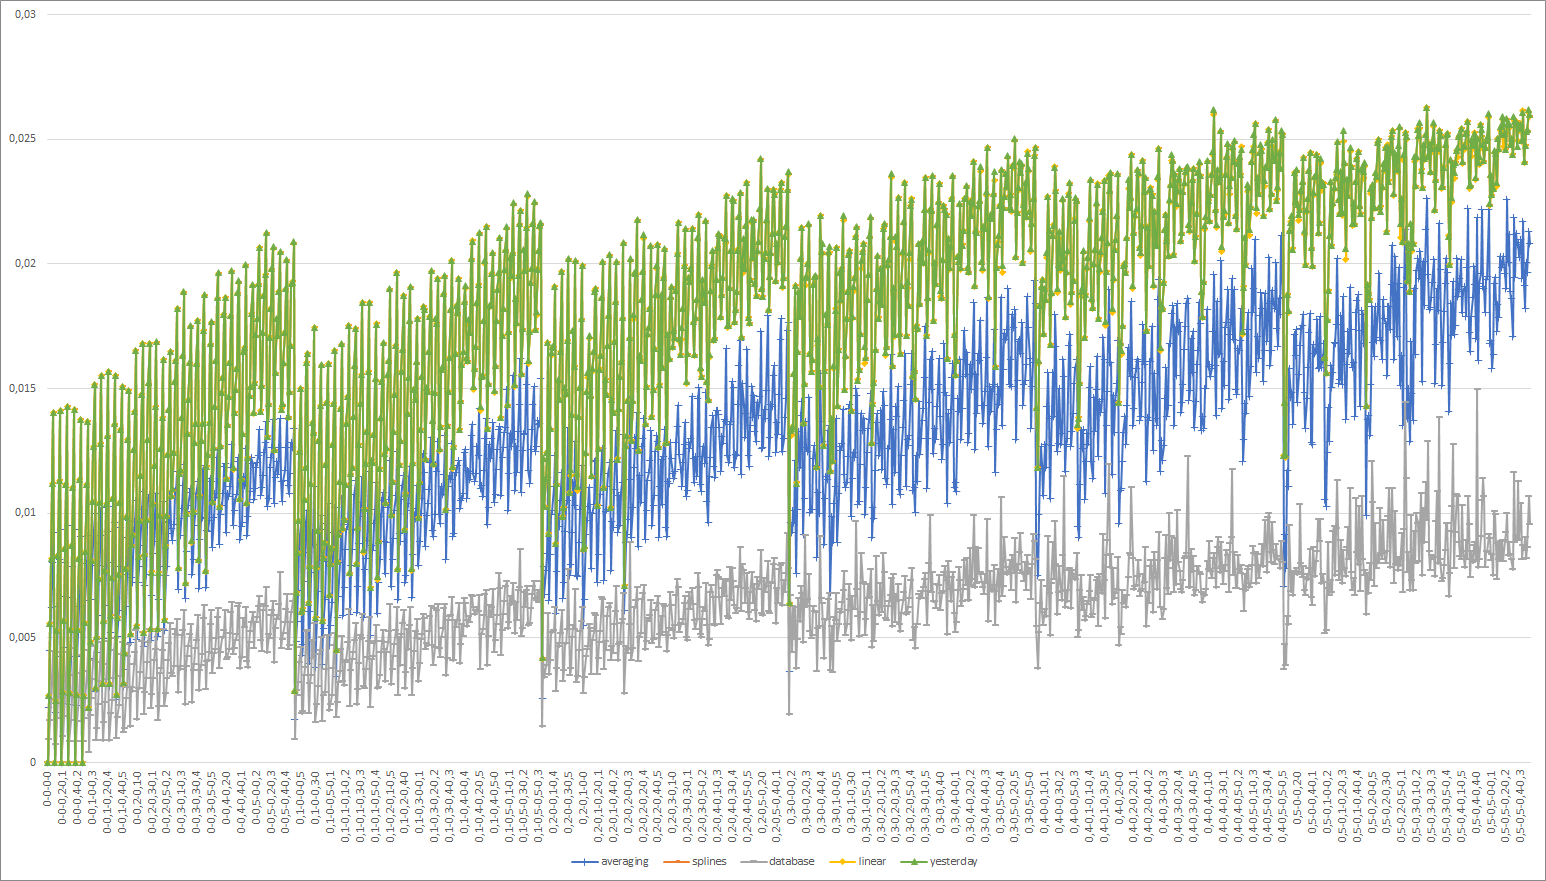
\includegraphics[width=0.9\columnwidth]{pics/evaluation-algorithms}
	\end{center}
	\caption{\label{fig:evaluation_algorithms}Gesamtergebnisse ohne Newton}
\end{figure}

Zunächst fällt auf, dass der Newton-Ansatz bei kleinen Lücken sehr gute Ergebnisse liefert, während sehr große Lücken in überaus hohen Distanzwerten resultieren. Dies liegt an der gebildeten Polynomfunktion, deren Werte bei großen Lücken in vielen Fällen stark nach oben oder unten ausreißt.
Die Bewertungen der anderen Algorithmen finden sich alle in einem vergleichsweise schmalen Bereich wieder, wie in Abbildung~\ref{fig:evaluation_algorithms} zu erkennen ist. Je mehr Daten fehlen, desto großer ist der Distanzwert. Dies gilt für alle Algorithmen. Die Werte innerhalb der Abbildung springen, da vier verschiedene Konfigurationsparameter auf eine Dimension reduziert werden mussten. Die fünf gleichmäßig verteilten Sprünge markieren die Stellen, an denen der Anteil entfernter Wochen zurückgesetzt wurde. Daraus resultierend sinkt der Anteil insgesamt entfernter Messwerte.
Der Test liefert sehr ähnliche Werte für die lineare Interpolation (in der Abbildung gelb), sowie für die Interpolation basierend auf Splines (orange) und den Daten des Vortages (Grün). Ein besseres Ergebnis liefert die Mittelwertinterpolation (blau). Innerhalb der sehr künstlichen Bedingungen liefert der Datenbankansatz (graue Werte) das beste Ergebnis.

\begin{figure}[!t]
	\begin{center}
		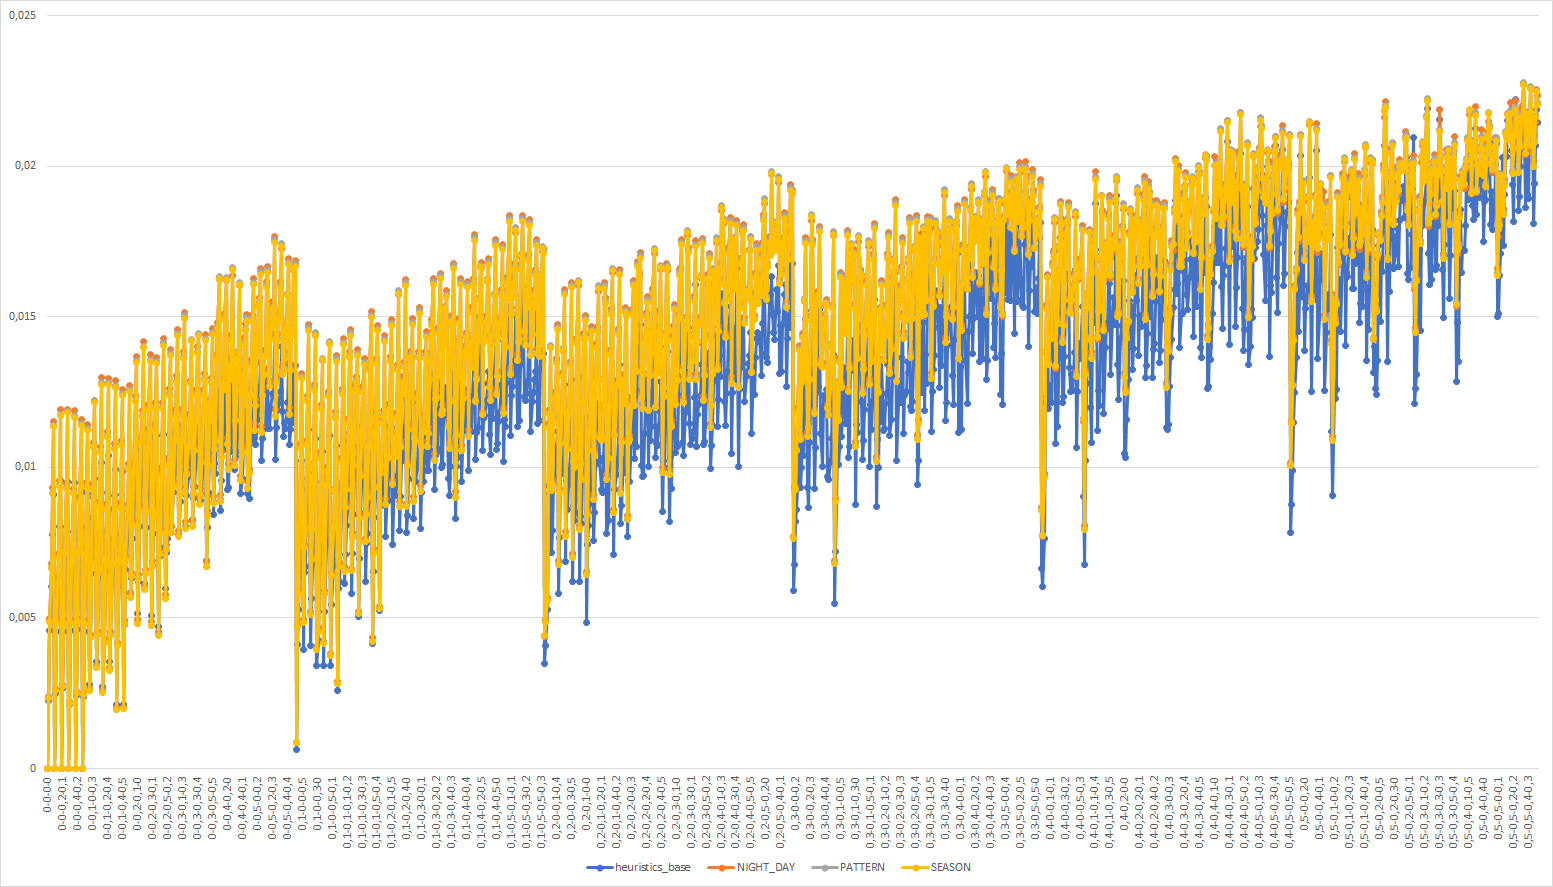
\includegraphics[width=0.9\columnwidth]{pics/evaluation-heuristics}
	\end{center}
	\caption{\label{fig:evaluation_heuristics}Gesamtergebnisse der Heuristiken}
\end{figure}

Als Basis für die Bewertung der Heuristiken dient ein mithilfe des Mittelwertverfahrens interpolierter Lastgang ebenfalls mit derselben Variation in den zufällig eingefügten Lücken. Wie in Abbildung~\ref{fig:evaluation_heuristics} zu erkennen ist, lässt sich ein ähnlicher Grundtrend wie bei den Algorithmen beobachten. Mit steigender Anzahl an Lücken nimmt der Distanzwert ebenfalls zu. Die drei Heuristiken produzieren dabei sehr ähnliche Ergebnisse, die in diesem Test leicht über den Werten der lediglich mit der Durchschnittsbildung interpolierten Basis liegen.
Die Verschlechterung ist zu beobachten, da die Ergebnisse der Mittelwertbildung ohne nachfolgende Interpolation ohnehin bereits sehr gut sind. In Verbindung mit anderen, schlechteren Interpolationsverfahren verbessern die Heuristiken die Ergebnisse. Dies gilt insbesondere für das Newton-Verfahren, dessen Bewertung sehr schlecht für größere Lücken ist. Mit nachfolgender Anwendung einer Heuristik verschiebt sich die Bewertung des Newton-Verfahrens in die Nähe der anderen Interpolationsverfahren.
Somit dienen die umgesetzten Heuristiken nicht der allgemeinen Verbesserung, sondern helfen bei der Validierung und daraus resultierenden Anpassung von Ausreißern, wie bei Newton beobachtet.

%!TEX root = ../paper.tex

\section{Ausblick}

Die Funktion und Validität der Algorithmen konnte mit der geringen Anzahl gegebener Testdatensätze nicht ausreichend genug getestet und sichergestellt werden.
Mit einer größeren Menge an verfügbaren Testdaten können insbesondere die Korrelationsmatrix und der Datenbankansatz bessere Ergebnisse liefern, da Einflüsse von Ausreißern in den verfügbaren Daten ausgeglichen und eine repräsentativere Datenbasis gebildet werden. Im Rahmen eines vollständigen Testprozesses müssen ebenfalls Sonderfälle abgedeckt und das Verhalten der Algorithmen und Heuristiken überprüft werden.

Im Rahmen der Evaluation wurden für die Konfigurationsparameter Werte verwendet, die nicht auf Basis von Fachwissen bestimmt wurden. Der Einfluss von tieferem und besseren Wissen durch Fachleute kann hierbei bereits die Ergebnisse verbessern oder zumindest realistischere Ergebnisse liefern.
Bestimmte Parameter, beispielsweise die Zusammenstellung der einfließenden Werte für die Mittelwertbildung, können möglicherweise ebenfalls gut durch einen Lernprozess bestimmt werden. Für die Mittelwertbildung ist hierzu ein Ansatz bereits implementiert, bei dem für unterschiedliche Abstände verschiedene Gewichtungen und Fensterbreiten getestet werden. Vergleichbar mit dem Testprozess wird der euklidische Abstand zwischen vollständigen Originaldaten und interpolierten Werten berechnet. Die Konfiguration, die den besten Abstandswert erzeugt, wird als Ergebnis gewählt, mit der im Weiteren interpoliert wird. Problematisch hierbei ist der benötige Rechenaufwand, der aus der Vielzahl an möglichen Kombinationen der Parameter resultiert. Möglicherweise kann der Lernprozess mit speziellen Algorithmen, bspw. einem Greedy-Algorithmus, beschleunigt werden. Es muss nicht zwingend die beste Konfiguration gefunden werden, eine gute Konfiguration reicht in der Regel aus. Lernverfahren für andere Algorithmen sind ebenso denkbar.

Die Algorithmen geben lediglich einfache Interpolationswerte aus. Zur Verbesserung der Interpretationsfähigkeit ist eine Ausgabe von Wahrscheinlichkeiten für die Werte hilfreich. Eine Erweiterung mit der Ausgabe verschiedener Werte mit unterschiedlicher Wahrscheinlichkeit ist ebenfalls denkbar, um verschiedene interpolierte Lastläufe anbieten zu können. Ein Anwender kann daraus basierend auf eigenen Einschätzungen oder tieferem, in den Algorithmen nicht abgebildetem Fachwissen die passendste Lösung auswählen.

Neuronale Netze und andere komplexere Algorithmen aus dem Themengebiet des Pattern Recognition sind ebenfalls denkbare Algorithmen. Alle im Rahmen des Projektes eingesetzten Algorithmen verarbeiten alle Interpolationen auf die gleiche Art. Komplexere Ansätze können so umgesetzt werden, dass sie unterschiedliche Bereiche auf verschiedene Art und Weise interpolieren. Entscheidungsgrundlage hierbei sind beispielsweise die Lückengröße oder Werteschwankungen innerhalb eines Analysefensters.
Anstatt einzelne, stark spezialisierte Algorithmen zu entwickeln, ist die Kombination verschiedener Algorithmen ebenfalls denkbar. Als Entscheidungsgrundlage können ebenfalls die genannten Kriterien verwendet werden.

% References	
%-----------------------------------------------------------------------
%\bibliographystyle{ieeetr}
%\bibliography{paper}


\end{document}

